\chapter{Deutsch–Jozsa Algorithm}

The Deutsch–Jozsa algorithm is a generalization of the Deutsch algorithm. It extends the problem from single-bit inputs to functions that take \( n \)-bit strings as inputs and return a single bit as output. This quantum algorithm provides an exponential speedup over classical counterparts by determining whether a given Boolean function is constant or balanced using only a single query to the oracle, as opposed to the \( O(2^{n-1}+1) \) queries required classically in the worst case.

\section{The Problem Definition}

\begin{definition}[Deutsch–Jozsa Problem]
Let \( f : \{0,1\}^n \rightarrow \{0,1\} \) be a Boolean function. The function \( f \) is said to be:
\begin{itemize}
    \item \textbf{Constant} if \( f(x) = 0 \) for all \( x \in \{0,1\}^n \) or \( f(x) = 1 \) for all \( x \in \{0,1\}^n \).
    \item \textbf{Balanced} if \( f(x) = 0 \) for exactly half of the inputs, and \( f(x) = 1 \) for the other half.
\end{itemize}
The promise is that \( f \) is either constant or balanced. The objective is to determine which of the two it is, using as few queries to the function \( f \) as possible.
\end{definition}

In classical computation, to be certain of the nature of \( f \), one might need to evaluate it on up to \( 2^{n-1} + 1 \) distinct inputs in the worst case. However, using quantum computation and the Deutsch–Jozsa algorithm, this problem can be solved with a single invocation of the quantum oracle \( U_f \).

The total number of possible Boolean functions from \( n \) input bits to a single output bit is \( 2^{2^n} \). Out of these, only \( 2 \) are constant functions, and the number of balanced functions is given by
\[
2 \times \binom{2^n}{2^{n-1}} = \frac{2(2^n)!}{(2^{n-1})!(2^n - 2^{n-1})!} \approx \sqrt{\frac{{2}}{\pi}}2^{2^n+1-n/2}.
\]
The rest of the functions are neither constant nor balanced.

As an illustrative case, consider \( n = 2 \). The possible functions are shown in Table~\ref{tab:Deutsch-jozsa}. We are given a black-box (oracle) computing a function that is promised to be either constant or balanced, but we are not told which one. Our goal is to determine whether the function is constant or balanced using as few queries to \( f \) as possible.

\begin{table}[ht]
    \centering
    \begin{subtable}[b]{0.45\linewidth}
        \centering
        \begin{tabular}{|c|c|c|}
            \hline
            Function & Input & Output \\
            \hline
            \( f_1 \) & 00 & 0 \\
                     & 01 & 0 \\
                     & 10 & 0 \\
                     & 11 & 0 \\
            \hline
            \( f_2 \) & 00 & 1 \\
                     & 01 & 1 \\
                     & 10 & 1 \\
                     & 11 & 1 \\
            \hline
        \end{tabular}
        \caption{Constant Functions}
    \end{subtable}%
    \hfill
    \begin{subtable}[b]{0.45\linewidth}
        \centering
        \begin{tabular}{|c|c|c|}
            \hline
            Function & Input & Output \\
            \hline
            \( f_3 \) & 00 & 0 \\
                     & 01 & 0 \\
                     & 10 & 1 \\
                     & 11 & 1 \\
            \hline
            \( f_4 \) & 00 & 0 \\
                     & 01 & 1 \\
                     & 10 & 1 \\
                     & 11 & 0 \\
            \hline
            \( \vdots \) & \( \vdots \) & \( \vdots \) \\
            \hline
            \( f_9 \) & 00 & 0 \\
                     & 01 & 1 \\
                     & 10 & 1 \\
                     & 11 & 0 \\
            \hline
        \end{tabular}
        \caption{Balanced Functions}
    \end{subtable}
    \caption{All possible constant and some balanced functions for \( n = 2 \).}
    \label{tab:Deutsch-jozsa}
\end{table}

\section{The Classical Solution}

\textbf{On a Classical Computer: } Note that even if you query the function in many spots and always see the same value, you still might not know which type of function it is. It could be constant, but it could also be that in the many places you did not query, the function takes the opposite value and is actually a balanced function. It is only after you've queried more than half of the input space that you can be sure about which case it is. 

Therefore, the number of queries that a classical algorithm must make is at least $2^{n-1} + 1$. In order to determine whether the function is constant or balanced, we need to query the function for just one more than half of the possible inputs.

Thus, we require $2^{n-1} + 1$ queries to determine with certainty whether the function is constant or balanced.

Hence, the time complexity on a classical computer is $\mathcal{O}(2^n)$, i.e., exponential time complexity in the number of input bits. That's a lot of queries when $n$ is large. If all the queried inputs produce the same output, we can conclude that the function is constant; otherwise, the function is balanced.

\begin{example}
Suppose that the problem is not to distinguish between the constant and balanced functions with certainty, but rather, with some probability of error $\epsilon < \frac{1}{2}$. What is the performance of the best classical algorithm for this problem?

Recall that a Boolean function $f : \{0,1\}^n \rightarrow \{0,1\}$ is said to be balanced if $f(x) = 1$ for exactly half of all possible $2^n$ values of $x$.

A single evaluation gives us no information about whether $f$ is constant or balanced, so our success rate (error rate) after a single evaluation is $\epsilon = \frac{1}{2}$ (random guessing!). 

Now consider the case where we do two evaluations. If we obtain two different results, then we can immediately conclude that $f$ is balanced.

Suppose instead that we obtain two results that are the same. If $f$ is balanced, then the probability that the first evaluation returns the given result is $\frac{1}{2}$, and the probability that the second evaluation returns the same result is
\[
\frac{2^{n-1} - 1}{2^n - 1}
\]
since there are $2^{n-1}$ inputs with each output (0 and 1), and after the first evaluation, only $2^{n-1} - 1$ matching values remain among the $2^n - 1$ remaining inputs.

Therefore, if $f$ is balanced, the probability of seeing the same result twice is
\[
\frac{1}{2} \cdot \frac{2^{n-1} - 1}{2^n - 1}
\]
which is less than $\frac{1}{2}$ as shown below:
\[
2^n < 2^{n+1} \Rightarrow 2^n - 2 < 2^{n+1} - 2 \Rightarrow \frac{2^{n-1} - 1}{2^n - 1} < 1 \Rightarrow \frac{1}{2} \cdot \frac{2^{n-1} - 1}{2^n - 1} < \frac{1}{2}
\]

Hence, if we get the same result in two evaluations, we can conclude that $f$ is constant with an error $\epsilon < \frac{1}{2}$. We conclude that only 2 evaluations are required for this classical probabilistic algorithm to achieve an error less than $1/2$.
\end{example}

\section{The Quantum Solution: Deutsch-Jozsa Algorithm}
\textbf{On a Quantum Computer:} To solve this problem, we need to query the function only once on a quantum computer using the Deutsch-Jozsa Algorithm. Thus, the time complexity to solve this problem is $\mathcal{O}(1)$, i.e., constant time complexity. This is an exponential speedup over the classical algorithm.

\subsection{Idea of the Algorithm}
Similar to the case of the Deutsch algorithm, we start off as usual, setting the target qubit to the state $\ket{-}$ and placing the other qubits — those which serve as inputs to $f$ — into a uniform superposition of all $n$-qubit states. This is achieved by applying a Hadamard gate to each of the $n$ qubits initially in the state $\ket{0}$, as shown in Figure~\ref{fig:deutsch-jozsa}. This results in phase kickback (also called querying in the phase) on all the qubits except the target qubit. Then, we apply a Hadamard transform on all the $n$ qubits to extract the phase difference. Finally, we perform a measurement which can clearly distinguish between the two cases: the function is \emph{constant} if the measurement reveals all $0$ in the classical state, and \emph{balanced} if the measurement reveals any non-zero value. Thus, we determine the nature of the function implemented inside the oracle.


\subsection{Algorithm}
The details are given in Algorithm~\ref{algo:deutsch_jozsa}.

\begin{algorithm}
    \caption{Deutsch-Jozsa Algorithm}
    \begin{algorithmic}[1]
    \State \textbf{Input:} A black box $U_f$ which performs the transformation $\ket{x}\ket{y} \rightarrow \ket{x}\ket{y \oplus f(x)}$, for $x \in \{0,\ldots,2^n - 1\}$ and $f(x) \in \{0,1\}$. It is promised that $f(x)$ is either constant for all values of $x$, or balanced, i.e., equal to $1$ for exactly half of all the possible $x$, and $0$ for the other half.
    \State \textbf{Output:} $0^n$ if and only if $f$ is constant.
    \State \textbf{Runtime:} One evaluation of $U_f$. Always succeeds.
    \State \textbf{Initialize:} $\ket{0^n}\ket{1}$
    \State Create superposition using Hadamard gates:
    \[
    \rightarrow \frac{1}{\sqrt{2^n}} \sum_{x=0}^{2^n - 1} \ket{x} \left(\frac{\ket{0} - \ket{1}}{\sqrt{2}}\right)
    \]
    \State Calculate function $f$ using $U_f$:
    \[
    \rightarrow \sum_x (-1)^{f(x)} \ket{x} \left(\frac{\ket{0} - \ket{1}}{\sqrt{2}}\right)
    \]
    \State Perform Hadamard transform:
    \[
    \rightarrow \sum_z \sum_x \frac{(-1)^{x \cdot z + f(x)} \ket{z}}{\sqrt{2^n}} \left(\frac{\ket{0} - \ket{1}}{\sqrt{2}}\right)
    \]
    \State Measure to obtain the final output $\ket{z}$
    \State If $z=0^n$ \textbf{return} constant or else return balanced.
    \end{algorithmic}
    \label{algo:deutsch_jozsa}
\end{algorithm}
The circuit for the Deutsch-Jozsa Algorithm is shown in Figure~\ref{fig:deutsch-jozsa}.

\begin{figure}[ht]
    \centering
    \begin{quantikz}
        \lstick{$\ket{0}$} & & \gate{H} & \gate[5]{U_f} & \gate{H} & \meter{} \\
        \lstick{$\ket{0}$} & & \gate{H} &              & \gate{H} & \meter{} \\
        &                  & \vdots    &              & \vdots   & \vdots   \\
        \lstick{$\ket{0}$} & & \gate{H} &              & \gate{H} & \meter{} \\
        \lstick{$\ket{0}$} & \gate{X}  &  \gate{H}            &          &         &
    \end{quantikz}
    \caption{Deutsch-Jozsa Circuit}
    \label{fig:deutsch-jozsa}
\end{figure}

The input of this circuit is $\ket{0^{n+1}}$. After applying the NOT gate on the last qubit, we have $\ket{0^n}\ket{1}$. The action of the Hadamard gate on the input will be:
\[
    H^{\otimes n}\ket{0}^{\otimes n}H\ket{1}=\frac{1}{\sqrt{2^n}}\sum_{x \in \{0,1\}^n}\ket{x}\frac{(\ket{0}-\ket{1})}{\sqrt{2}}
\]
Now, the oracle will show the action $U_f$ as $U_f\ket{x}\ket{y}=\ket{x}\ket{y \oplus f(x)}$ (here $x \in \{0,1\}^n$), and thus the action of the oracle will be:
\begin{align*}
    U_f\left(\frac{1}{\sqrt{2^n}}\sum_{x \in \{0,1\}^n}\ket{x}\frac{(\ket{0}-\ket{1})}{\sqrt{2}}\right)
    &=U_f\left(\frac{1}{\sqrt{2^n}}\frac{1}{\sqrt{2}}\sum_{x \in \{0,1\}^n} \left( \ket{x}\ket{0}-\ket{x}\ket{1} \right) \right)\\
    &=\frac{1}{\sqrt{2^n}}\frac{1}{\sqrt{2}}\sum_{x \in \{0,1\}^n} \left( U_f\ket{x}\ket{0} - U_f\ket{x}\ket{1} \right)\\
    &=\frac{1}{\sqrt{2^n}}\sum_{x \in \{0,1\}^n}\ket{x}\left(\frac{\ket{0 \oplus f(x)} - \ket{1 \oplus f(x)}}{\sqrt{2}}\right)
\end{align*}

Now, $\ket{0 \oplus f(x)}=\ket{f(x)}$ and $\ket{1 \oplus f(x)} = \ket{\overline{f(x)}}$, where $\overline{f(x)}$ is the complement of $f(x)$. Thus, substituting this into the equation, we get:
\[
    \frac{1}{\sqrt{2^n}}\sum_{x \in \{0,1\}^n}\ket{x}\left(\frac{\ket{f(x)} - \ket{\overline{f(x)}}}{\sqrt{2}}\right)
\] 
Now, when $f(x)=0$ then 
\[
\frac{\ket{f(x)} - \ket{\overline{f(x)}}}{\sqrt{2}} = \frac{\ket{0} - \ket{1}}{\sqrt{2}} = \ket{-}
\]
and when $f(x)=1$ then
\[
\frac{\ket{f(x)} - \ket{\overline{f(x)}}}{\sqrt{2}} = \frac{\ket{1} - \ket{0}}{\sqrt{2}} = -\ket{-}.
\]
Thus, this can be written as: 
\[
    \frac{1}{\sqrt{2^n}}\sum_{x \in \{0,1\}^n}(-1)^{f(x)}\ket{x}\ket{-}
\]
Note that the first $n$ qubits form a uniform superposition of all $2^n$ computational basis states of $n$ qubits, with a phase of $(-1)^{f(x)}$ for each $\ket{x}$.  

Now, we apply the Hadamard gate on the first $n$ qubits. In the constant case, this transforms the state to $\pm \ket{00\ldots 0} = \pm \ket{0^n}$. In the balanced case, since unitary operations preserve orthogonality relationships, the state is transformed to some state that is orthogonal to $\ket{0^n}$. Thus, the action of the Hadamard gate on these qubits will be:
\begin{align*}
    (H^{\otimes n}\otimes I)\left(\frac{1}{\sqrt{2^n}}\sum_{x \in \{0,1\}^n}(-1)^{f(x)}\ket{x}\ket{-}\right)
    &=H^{\otimes n}\left(\frac{1}{\sqrt{2^n}}\sum_{x \in \{0,1\}^n}(-1)^{f(x)}\ket{x}\right) \otimes I\ket{-}\\
    &=\left(\frac{1}{\sqrt{2^n}}\sum_{x \in \{0,1\}^n}(-1)^{f(x)}H^{\otimes n}\ket{x}\right) \otimes \ket{-}
\end{align*}

Recall that $H^{\otimes n}\ket{x}=\dfrac{1}{\sqrt{2^n}}\sum_{y \in \{0,1\}^n}(-1)^{x\cdot y}\ket{y}$ for the Hadamard gate (refer to Section~\ref{qgate:hadamard}) acting on $n$ qubits. Thus, substituting this into the above equation, we can write:
\[
    \left(\frac{1}{2^n}\sum_{x \in \{0,1\}^n}\sum_{y \in \{0,1\}^n}(-1)^{f(x)+x\cdot y}\ket{y}\right) \otimes \ket{-}
\]

Now, we perform the measurement on the first $n$ qubits. All we really care about is the probability that the measurements all give outcome $0$. The amplitude associated with the classical state $\ket{0^n}$ is
\[
\dfrac{1}{2^n}\sum_{x\in\{0,1\}^n} (-1)^{f(x)}.
\]
Thus, the probability that the measurement gives outcome $0$ for all qubits is
\[
\left|\dfrac{1}{2^n} \sum_{x\in\{0,1\}^n}
(-1)^{f(x)}\right|^2 = 
\begin{cases} 
1 & \text{if $f$ is constant}, \\
0 & \text{if $f$ is balanced}.
\end{cases}
\]



In the constant case, either all the phases are $+1$ or all the phases are $-1$. So the state remains in a uniform superposition of computational basis states and just picks up a global phase of $+1$ or $-1$. In the balanced case, there are lots of possibilities, depending on which particular balanced function it is. But one thing we can say is that the state is orthogonal to the state that arises in the constant case. Because, in the computational basis, the state will have $+1$ in half of its components and $-1$ in the other half. So when you take the dot product with a vector that has (say) $+1$ in each component, you get an equal number of $+1$s and $-1$s, which cancel and result in zero.

Note that since the cases we are trying to distinguish between result in orthogonal states, in principle, they are perfectly distinguishable.

Consider the following two cases:
\begin{enumerate}
    \item \textbf{Case 1: Function is Constant}
    \begin{itemize}
        \item Let $f(x)=0$ for all $x \in \{0,1\}^n$. Hence we need to perform measurement on the first n qubits of the following state:
        \[
            \left(\frac{1}{2^n}\sum_{x \in \{0,1\}^n}\sum_{y \in \{0,1\}^n}(-1)^{x\cdot y}\ket{y}\right)\otimes \ket{-}
        \]
        Upon simplifying we get,
        \[
            \left(\frac{1}{2^n}2^n\ket{0^{\otimes n}}\right)\otimes \ket{-} = \ket{0^{\otimes n}} \otimes \ket{-}
        \]
        Thus, upon measurement the output will be $\ket{0^{\otimes n}}$ with probability $1$. Thus, we get a measurement of $\ket{0^{\otimes n}}$.
        \item Let $f(x)=1$ for all $x \in \{0,1\}^n$. Hence we need to perform measurement on the first n qubits of the following state:
        \[
            \left(\frac{1}{2^n}\sum_{x \in \{0,1\}^n}\sum_{y \in \{0,1\}^n}(-1)^{1+x\cdot y}\ket{y}\right)\otimes \ket{-}
        \]
        Upon simplifying we get,
        \[
            \left(\frac{1}{2^n}2^n\ket{0^{\otimes n}}\right)\otimes \ket{-} = -\ket{0^{\otimes n}} \otimes \ket{-}
        \]
        Thus, upon measurement the output will be $\ket{0^{\otimes n}}$ with probability $1$. Thus, we get a measurement of $\ket{0^{\otimes n}}$.
    \end{itemize}
    \item \textbf{Case 2: Function is Balanced}
    \begin{itemize}
        \item Let $f(x)$ be a balanced function. Thus, $f(x)=0$ for exactly half of the inputs and $f(x)=1$ for the other half of the inputs. Hence we need to perform measurement on the first n qubits of the following state:
        \[
            \left(\frac{1}{2^n}\sum_{x \in \{0,1\}^n}\sum_{y \in \{0,1\}^n}(-1)^{f(x)+x\cdot y}\ket{y}\right)\otimes \ket{-}
        \]
        The output of this depends on the function but it will surely not be $\ket{0^n}$.
    \end{itemize}
     If the outcome is $00.\ldots 0=0^n$ then we report "constant" and if the outcome is any string that's not $0^n$ (not all zeroes) then we report "balanced". Note that in the balanced case, it is impossible to get outcome $0^n$, because measuring a state orthogonal to $0^n$ cannot result in outcome $0^n$.

     Thus, the one-query algorithm for the constant vs balanced problem works. It achieves something with one single query that requires exponentially many queries by any classical algorithm.
\end{enumerate}

\subsection{Example}
\begin{example}
    \begin{figure}[ht]
        \centering
        \begin{quantikz}
            \lstick{$\ket{0}$} & & \gate{H} & \gate[3]{U_f} & \gate{H} & \meter{}\\
            \lstick{$\ket{0}$} & & \gate{H} & & \gate{H} & \meter{}\\
            \lstick{$\ket{0}$} & \gate{X} & \gate{H} & & &
        \end{quantikz}
        \caption{Deutsch-Jozsa circuit for $n=2$}
        \label{fig:deutsch-jozsaex}
    \end{figure}
    Consider the Deutsch-Jozsa algorithm for $n=2$. The possible functions are as shown in Table~\ref{tab:Deutsch-jozsa}, and the circuit for the Deutsch-Jozsa algorithm is shown in Figure~\ref{fig:deutsch-jozsaex}. 
    The input to the circuit is $\ket{00}\ket{1}$. The action of the Hadamard gate on the input will be:
    \begin{align*}
        H^{\otimes 2}\ket{00}H\ket{1}&=\frac{1}{2}\sum_{x\in \{0,1\}^2}\ket{x}\frac{\ket{0}-\ket{1}}{\sqrt{2}} \\
        &=\frac{1}{2\sqrt{2}}\left(\ket{000}+\ket{010}+\ket{100}+\ket{110}-\ket{001}-\ket{011}-\ket{101}-\ket{111}\right)
    \end{align*}
    The action of the oracle will be:
    \begin{align*}
        &U_f\left(\frac{1}{2\sqrt{2}}(\ket{000}+\ket{010}+\ket{100}+\ket{110}-\ket{001}-\ket{011}-\ket{101}-\ket{111})\right)\\
        &=\frac{1}{2\sqrt{2}}(U_f\ket{000}+U_f\ket{010}+U_f\ket{100}+U_f\ket{110}-U_f\ket{001}-U_f\ket{011}-U_f\ket{101}-U_f\ket{111})\\
        &=\frac{1}{2\sqrt{2}}(\ket{00}\ket{f(00)}+\ket{01}\ket{f(01)}+\ket{10}\ket{f(10)}+\ket{11}\ket{f(11)}-\ket{00}\ket{\overline{f(00)}}
    \end{align*}
    \[
    -\ket{01}\ket{\overline{f(01)}}-\ket{10}\ket{\overline{f(10)}}-\ket{11}\ket{\overline{f(11)}})
    \]

    Now consider the following cases:
\begin{enumerate}
    \item \textbf{Case 1: $f(x)$ is constant}\\
    \begin{itemize}
        \item Let $f(x)=0$ for all $x \in \{0,1\}^2$. Thus, the output of the oracle will be:
        \begin{align*}
            &\frac{1}{2\sqrt{2}}(\ket{00}\ket{0}+\ket{01}\ket{0}+\ket{10}\ket{0}+\ket{11}\ket{0}-\ket{00}\ket{1}-\ket{01}\ket{1}-\ket{10}\ket{1}-\ket{11}\ket{1})\\
            &=\frac{1}{2\sqrt{2}}(\ket{000}+\ket{010}+\ket{100}+\ket{110}-\ket{001}-\ket{011}-\ket{101}-\ket{111})\\
            &=\frac{1}{2}(\ket{00}+\ket{01}+\ket{10}+\ket{11})\otimes \frac{\ket{0}-\ket{1}}{\sqrt{2}}
        \end{align*}
        Now we apply the Hadamard on the first $n$ qubits, and we get:
        \begin{align*}
            &(H^{\otimes 2}\otimes I)\frac{1}{2}((\ket{00}+\ket{01}+\ket{10}+\ket{11})\otimes \ket{-})\\
            &=\frac{1}{2}(H^{\otimes 2}\ket{00}+H^{\otimes 2}\ket{01}+H^{\otimes 2}\ket{10}+H^{\otimes 2}\ket{11})\otimes \ket{-}\\
            &=\frac{1}{2}[\frac{1}{2}(\ket{00}+\ket{01}+\ket{10}+\ket{11})+\frac{1}{2}(\ket{00}-\ket{01}+\ket{10}-\ket{11})]
        \end{align*}
        Upon simplifying, we get:
        \[
            \frac{1}{4}(4\ket{00})\otimes \ket{-}=\ket{00}\otimes \ket{-}
        \]
        Thus, upon measurement, the output will be $\ket{00}$ with probability $1$. Therefore, we get a measurement of $\ket{00}$.

        \item Let $f(x)=1$ for all $x \in \{0,1\}^2$. Thus, the output of the oracle will be:
        \begin{align*}
            &\frac{1}{2\sqrt{2}}(\ket{00}\ket{1}+\ket{01}\ket{1}+\ket{10}\ket{1}+\ket{11}\ket{1}-\ket{00}\ket{0}-\ket{01}\ket{0}-\ket{10}\ket{0}-\ket{11}\ket{0})\\
            &=\frac{-1}{2\sqrt{2}}(\ket{000}+\ket{010}+\ket{100}+\ket{110}-\ket{001}-\ket{011}-\ket{101}-\ket{111})\\
            &=\frac{-1}{2}(\ket{00}+\ket{01}+\ket{10}+\ket{11})\otimes \frac{\ket{0}-\ket{1}}{\sqrt{2}}
        \end{align*}
        Now we apply the Hadamard on the first $n$ qubits, and we get:
        \begin{align*}
            &(H^{\otimes 2}\otimes I)\frac{-1}{2}((\ket{00}+\ket{01}+\ket{10}+\ket{11})\otimes \ket{-})\\
            &=\frac{-1}{2}(H^{\otimes 2}\ket{00}+H^{\otimes 2}\ket{01}+H^{\otimes 2}\ket{10}+H^{\otimes 2}\ket{11})\otimes \ket{-}\\
            &=\frac{-1}{2}[\frac{1}{2}(\ket{00}+\ket{01}+\ket{10}+\ket{11})+\frac{1}{2}(\ket{00}-\ket{01}+\ket{10}-\ket{11})\\
            &\quad +\frac{1}{2}(\ket{00}+\ket{01}-\ket{10}-\ket{11})+\frac{1}{2}(\ket{00}-\ket{01}-\ket{10}+\ket{11})]\otimes \ket{-}
        \end{align*}
        Upon simplifying, we get:
        \[
            \frac{-1}{4}(4\ket{00})\otimes \ket{-}=\ket{00}\otimes -\ket{-}
        \]
        Thus, upon measurement, the output will be $\ket{00}$ with probability $1$. Therefore, we get a measurement of $\ket{00}$.
    \end{itemize}

    \item \textbf{Case 2: $f(x)$ is balanced}\\
    \begin{itemize}
        \item Let $f(x)$ be a balanced function. Thus, $f(x)=0$ for exactly half of the inputs and $f(x)=1$ for the other half of the inputs.  
        Then it can be shown that, based on the input chosen, the output will be either of the first $n$ qubits, $\ket{11}$ or $-\ket{11}$.  
        Thus, upon measurement, the output will be $\ket{11}$ with probability $1$. Therefore, we get a measurement of $\ket{11}$.
    \end{itemize}
\end{enumerate}
\end{example}

\section{Complexity Analysis}

Note that the classical query cost is expensive only if we require absolutely perfect performance. If a classical procedure queries $f$ at random inputs, then in the case of a balanced function, it would have to be very unlucky to draw the same output value twice.

Here is a classical probabilistic procedure that makes just two queries and performs reasonably well. It selects two inputs randomly (independently), and then outputs ``constant'' if the two outputs are the same and ``balanced'' if the two outputs are different.

\begin{itemize}
    \item If $f$ is constant, then the algorithm always succeeds.
    \item If $f$ is balanced, the algorithm succeeds with probability $\frac{1}{2}$, since the probability of choosing two inputs that yield different outputs is $\frac{1}{2}$.
\end{itemize}

By repeating the above procedure $k$ times, we can make the error probability exponentially small in $k$. For instance, only 4 queries are needed to achieve a success probability of $\frac{3}{4}$. The success probability can be made arbitrarily close to 1 using a constant number of queries.

In summary, we have considered three problems in the black-box model. For each problem, a quantum algorithm solves it with just one query, while classical algorithms—whether deterministic or probabilistic—require more:

\begin{table}[ht]
    \centering
    \begin{tabular}{|c|c|c|c|}
        \hline
        \textbf{Problem} & \textbf{Quantum Solution} & \textbf{Classical Deterministic} & \textbf{Classical Probabilistic} \\
        \hline
        Deutsch & 1 & 2 & 2 \\
        \hline
        Deutsch-Jozsa & 1 & $2^{n-1} + 1$ & $\mathcal{O}(1)$ \\
        \hline
    \end{tabular}
    \caption{Summary of query complexity for the considered problems}
    \label{tab:deutsch_querycost}
\end{table}

For the Deutsch problem, any classical algorithm requires 2 queries. For the Deutsch-Jozsa problem, a deterministic classical algorithm requires exponentially many queries to solve the problem with certainty. However, a probabilistic classical algorithm can solve the problem with bounded error using only a constant number of queries.

This raises a natural question: \emph{Is there a black-box problem where even probabilistic classical algorithms with bounded-error probability require exponentially more queries than a quantum algorithm?}

Such problems seem somewhat contrived and lack immediate practical relevance. Nevertheless, this line of inquiry is critical for understanding the potential of quantum advantage. Up to this point, we have not yet demonstrated a significant advantage of quantum algorithms over probabilistic classical algorithms. We will address this in the next chapter.

\section{Conclusion}

From the Deutsch-Jozsa algorithm, it is evident that to determine whether the function $f:\{0,1\}^n \rightarrow \{0,1\}$ is constant or balanced, we prepare the input state with $n$ qubits in the state $\ket{0}$ and one target qubit in the state $\ket{1}$. Then, by querying the function only once, we apply Hadamard transforms before and after the oracle call.

Upon final measurement of the first $n$ qubits:
\begin{itemize}
    \item If the result is $\ket{0}^{\otimes n}$, then the function is constant.
    \item If the result is orthogonal to $\ket{0}^{\otimes n}$, then the function is balanced.
\end{itemize}

Thus, we can determine whether the function is constant or balanced with just \textbf{one query} to the oracle. This gives the Deutsch-Jozsa algorithm a \textbf{time complexity of} $\mathcal{O}(1)$—an exponential speedup over the best classical deterministic algorithm, which requires $2^{n-1} + 1$ queries.

\section{Implementation using Qiskit}
\subsection{Background}
Usage estimate: 4 seconds on \texttt{ibm\_brisbane} (NOTE: This is an estimate only. Your runtime may vary).\\
To run the Deutsch-Jozsa algorithm, an oracle is required that implements a function which is either constant or balanced, along with the Deutsch-Jozsa circuit.

Here, we demonstrate how to construct Deutsch-Jozsa oracles and use the gates from the Qiskit circuit library to easily set up a Deutsch-Jozsa circuit.

\subsection{Requirements}
Before starting this tutorial, ensure that you have the following installed:
\begin{itemize}
    \item Qiskit SDK 1.0 or later, with visualization support (\texttt{pip install 'qiskit[visualization]'})
    \item Qiskit Runtime 0.22 or later (\texttt{pip install qiskit-ibm-runtime})
\end{itemize}

\subsection{Setup}
Here we import the small number of tools needed for this tutorial.
\begin{lstlisting}[language=Python]
#Built-in modules
import math

#imports from Qiskit
from qiskit import QuantumCircuit, QuantumRegister, ClassicalRegister
from qiskit.visualization import plot_histogram
from qiskit_aer import AerSimulator

#Imports from Qiskit Primitives
from qiskit_ibm_runtime import SamplerV2 as Sampler

#Imports from Qiskit Runtime
from qiskit_ibm_runtime import QiskitRuntimeService
\end{lstlisting}

\begin{lstlisting}[language=Python]
# backend = AerSimulator()  # Use AerSimulator for local simulation

# To run on IBM Quantum hardware
service = QiskitRuntimeService(channel="ibm_quantum")
backend = service.least_busy(operational=True, simulator=False)
backend.name
\end{lstlisting}

This will output one of the IBM Quantum computers (e.g., \texttt{ibm\_brisbane}).

\begin{enumerate}
    \item \textbf{Step 1: Map classical inputs to a quantum problem}: \\
    Deutsch-Jozsa algorithm requires an oracle that implements the function either constant or balanced. Here, we demonstrate how to construct Deutsch-Jozsa oracles and use the gates from the Qiskit circuit library to easily set up a Deutsch-Jozsa Circuit. Here, we will work the  with 2 qubits for constant and balanced functions and verify the results as expected.

The runtime Sampler primitive allows seamless execution of Deutsch-Jozsa circuit.
\begin{lstlisting}[language=Python]
def deutsch_jozsa(num_qubits=2,value=0,oracle_type="constant",b_str=""):
    # Create a Quantum Circuit
    qubits=QuantumRegister(num_qubits+1,name="q")
    cbits=ClassicalRegister(num_qubits,name="c")
    circuit=QuantumCircuit(qubits,cbits)

    circuit.x(qubits[-1])

    for qubit in qubits:
        circuit.h(qubit)
    
    circuit.barrier()

    oracle_qc=QuantumRegister(num_qubits+1)
    oracle=QuantumCircuit(oracle_qc,name="Oracle")
    if(oracle_type=="constant"):
        if(value==1):
            oracle.x(oracle_qc[-1])
            oracle.name="Const Oracle: 1"
        elif(value==0):
            oracle.id(oracle_qc[-1])
            oracle.name="Const Oracle: 0"
        else:
            raise ValueError("Value must be 0 or 1")
    elif(oracle_type=="balanced"):
        if(b_str==""):
            raise ValueError("Balanced Oracle requires a bit string")
        if(len(b_str)!=num_qubits):
            raise ValueError("Bit string must be of length equal to number of qubits")
        for qubit in range(num_qubits):
            if(b_str[qubit]=="1"):
                oracle.x(oracle_qc[qubit])
        
        for qubit in oracle_qc[:-1]:
            oracle.cx(qubit,oracle_qc[-1])

        for qubit in range(num_qubits):
            if(b_str[qubit]=="1"):
                oracle.x(oracle_qc[qubit])
        oracle.name="Balanced Oracle"
    else:
        raise ValueError("Oracle type must be 'constant' or 'balanced'")
            
    circuit.append(oracle, qubits)
            
    circuit.barrier()

    for qubit in qubits[:-1]:
        circuit.h(qubit)

    for qubit in qubits[:-1]:
        circuit.measure(qubit,qubits.index(qubit))

    return circuit
\end{lstlisting}
    Note the above code can create only certain type o balanced functions and not all its variants. For creating the function $f=f_3$, the following code is used.
    \begin{lstlisting}[language=Python]
# Create a Quantum Circuit
qubits = QuantumRegister(3, name="q")
cbits = ClassicalRegister(2, name="c")
circuit = QuantumCircuit(qubits, cbits)

q0, q1, q2 = qubits
circuit.h(q0)
circuit.h(q1)
circuit.x(q2)
circuit.h(q2)

circuit.barrier()

# Oracle implementation for f = f3 (example)
circuit.cx(q0, q2)

circuit.barrier()

circuit.h(q0)
circuit.h(q1)
circuit.measure(q0, cbits[0])
circuit.measure(q1, cbits[1])

circuit.draw("mpl")
\end{lstlisting}

The rest of the code corresponding to $f = f_3$ follows a similar pattern.

For creating a constant oracle circuit, use the following code:

\begin{lstlisting}[language=Python]
qc_const_0 = deutsch_jozsa(num_qubits=2, value=0, oracle=True, oracle_type="constant", b_str="00")
qc_const_0.draw("mpl")
\end{lstlisting}

For a balanced oracle, the code used is as follows:

\begin{lstlisting}[language=Python]
qc_bal_0 = deutsch_jozsa(num_qubits=2, value=1, oracle=True, oracle_type="balanced", b_str="00")
qc_bal_0.draw("mpl")
\end{lstlisting}

Similarly, any other circuit can be created by changing the input parameters.

The circuit along with the corresponding oracle implementing the function is shown in Figure~\ref{fig:deutsch-jozsa_circuit}, corresponding to the functions listed in Table~\ref{tab:Deutsch-jozsa}.

     \begin{figure}[ht]
    \centering
    \begin{subfigure}[b]{0.45\linewidth}
        \centering
        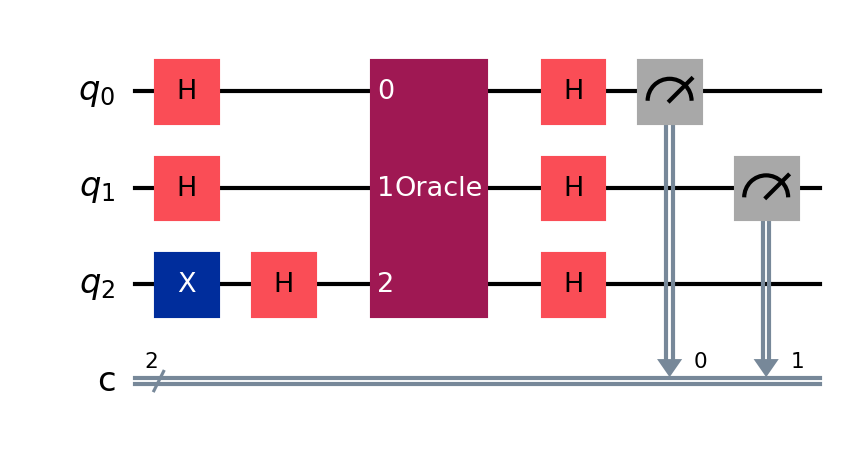
\includegraphics[width=\linewidth]{Images/deutsch_const_0.png}
        \caption{$f = f_1$ (Constant)}
        \label{fig:deutsch_jozsa_f1}
    \end{subfigure}
    \hfill
    \begin{subfigure}[b]{0.45\linewidth}
        \centering
        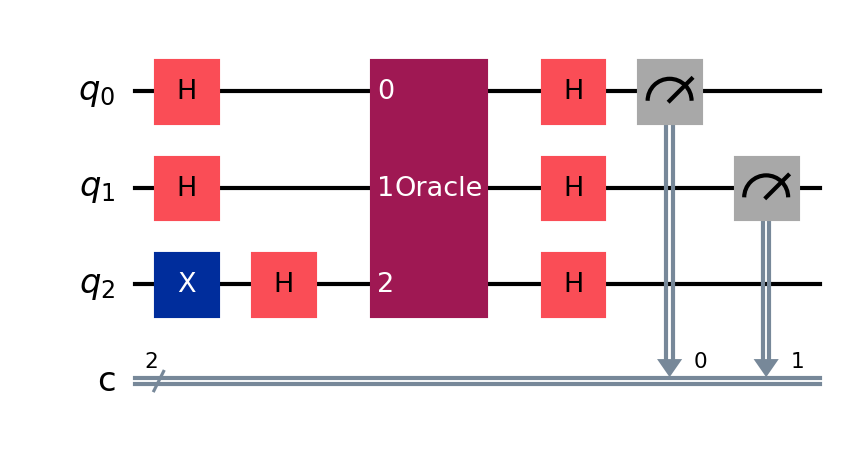
\includegraphics[width=\linewidth]{Images/deutsch_const_1.png}
        \caption{$f = f_2$ (Constant)}
        \label{fig:deutsch_jozsa_f2}
    \end{subfigure}
    
    \vspace{0.5cm}
    
    \begin{subfigure}[b]{0.45\linewidth}
        \centering
        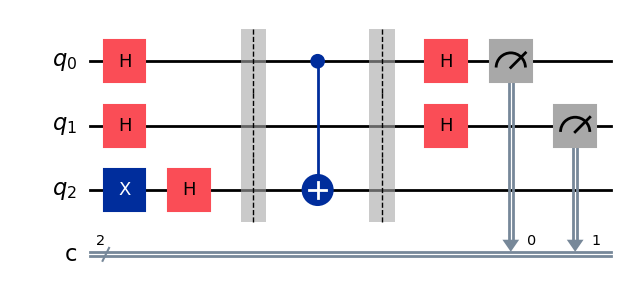
\includegraphics[width=\linewidth]{Images/deutsch_jozsa_bal_0.png}
        \caption{$f = f_3$ (Balanced)}
        \label{fig:deutsch_jozsa_f3}
    \end{subfigure}
    \hfill
    \begin{subfigure}[b]{0.45\linewidth}
        \centering
        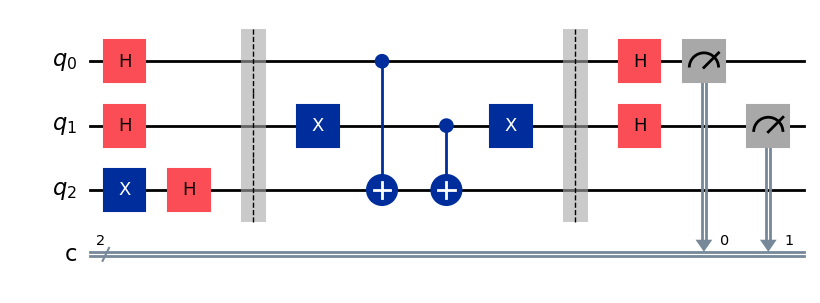
\includegraphics[width=\linewidth]{Images/deutsch_jozsa_bal_1.png}
        \caption{$f = f_4$ (Balanced)}
        \label{fig:deutsch_jozsa_f4}
    \end{subfigure}
    
    \caption{Deutsch-Jozsa circuit implementations for a few of the possible functions, along with their corresponding oracles.}
    \label{fig:deutsch-jozsa_circuit}
\end{figure}

Note that the oracle (shown between the two barriers) implements the required functions. Thus, the above figure corresponds to the Deutsch-Jozsa circuit with a few representative functions.

\item \textbf{Step 2: Optimize Problems for Quantum Execution}

\begin{lstlisting}[language=Python]
target=backend.target
pm = generate_preset_pass_manager(backend=backend, optimization_level=3)

circuit_isa_const_0=pm.run(qc_const_0)
circuit_isa_const_0.draw(output="mpl")
\end{lstlisting}


\begin{figure}[ht]
    \centering
    \begin{subfigure}[b]{0.45\linewidth}
        \centering
        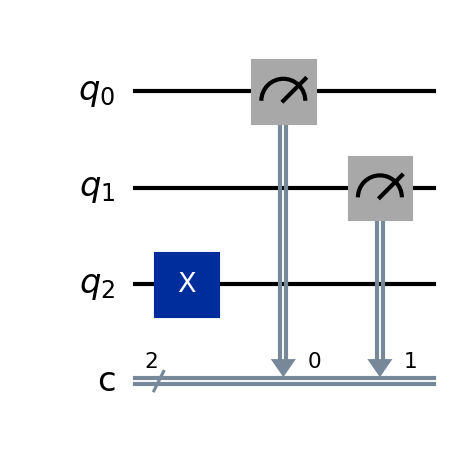
\includegraphics[width=\linewidth]{Images/deutsch_const_opt_0.png}
        \caption{$f = f_1$ (Constant)}
        \label{fig:deutsch_const_opt_f1}
    \end{subfigure}
    \hfill
    \begin{subfigure}[b]{0.45\linewidth}
        \centering
        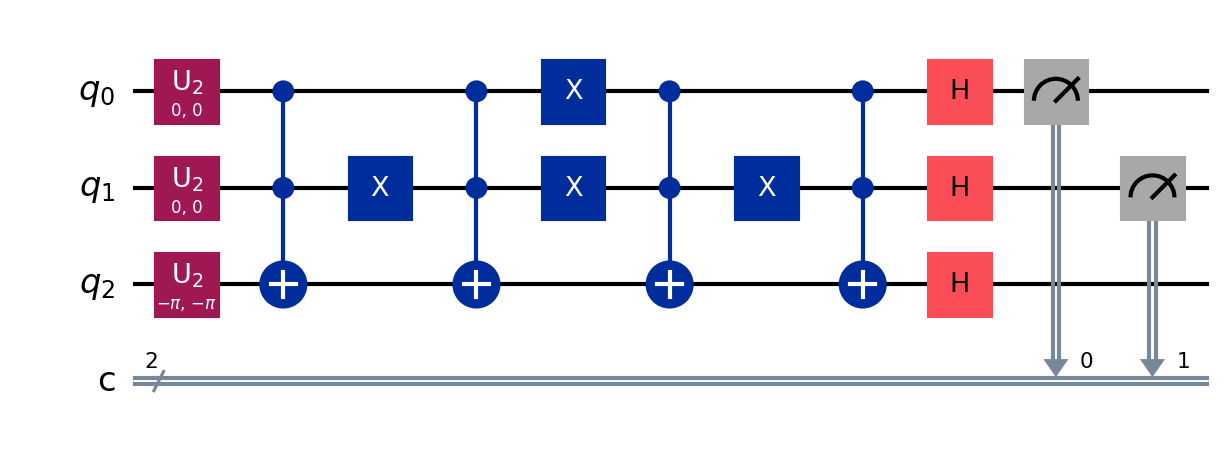
\includegraphics[width=\linewidth]{Images/deutsch_const_opt_1.png}
        \caption{$f = f_2$ (Constant)}
        \label{fig:deutsch_const_opt_f2}
    \end{subfigure}
    
    \vspace{0.5cm}
    
    \begin{subfigure}[b]{0.45\linewidth}
        \centering
        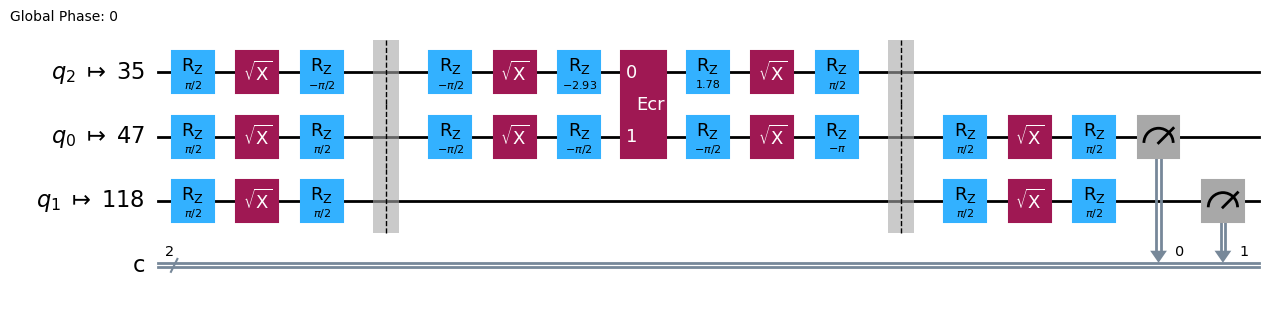
\includegraphics[width=\linewidth]{Images/deutsch_jozsa_bal_opt_0.png}
        \caption{$f = f_3$ (Balanced)}
        \label{fig:deutsch_jozsa_bal_opt_0}
    \end{subfigure}
    \hfill
    \begin{subfigure}[b]{0.45\linewidth}
        \centering
        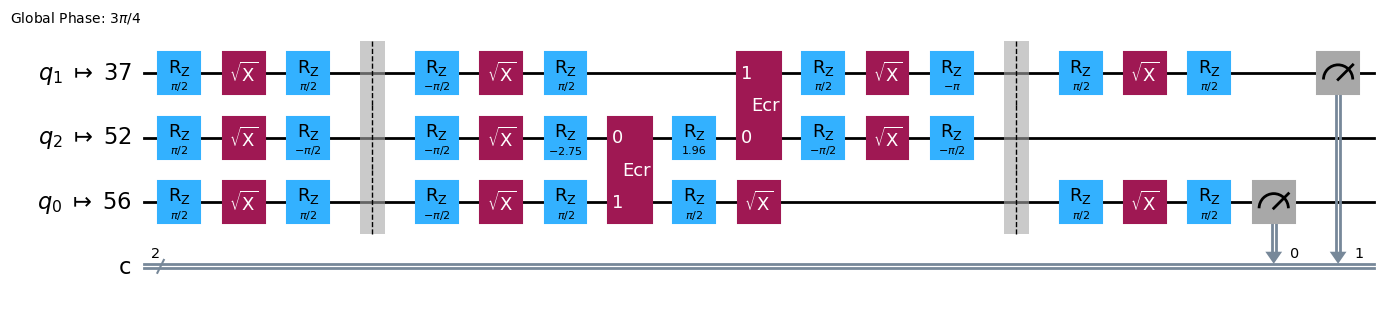
\includegraphics[width=\linewidth]{Images/deutsch_jozsa_bal_opt_1.png}
        \caption{$f = f_4$ (Balanced)}
        \label{fig:deutsch_jozsa_bal_opt_1}
    \end{subfigure}
    
    \caption{Optimized Deutsch-Jozsa circuit implementations for possible functions, along with their corresponding oracles.}
    \label{fig:deutsch-jozsa_opt_circuit}
\end{figure}

The optimized circuits shown in Figure~\ref{fig:deutsch-jozsa_opt_circuit} are the ones that actually get executed on a quantum computer, as they are optimized for the target hardware.

    \item \textbf{Step 3: Execute using Qiskit Primitives} \\
    We now run the circuit and sample the measurements on the first qubit. For execution, we use the \texttt{Sampler} runtime primitive.
    
\begin{lstlisting}[language=Python]
sampler=Sampler(mode=backend)
sampler.options.default_shots=10_000
result_const_0 = sampler.run([circuit_isa_const_0]).result()
dist_const_0 = result_const_0[0].data.c.get_counts()
\end{lstlisting}
    
    The output of the above code will be the distribution of measurements on the first two qubits. Similar code can be written for all other possible functions by just implementing the required oracle.
    
    \item \textbf{Step 4: Post-Process Results} \\
    Now we plot a histogram of the measurements on the first two qubits in classical format.
    
\begin{lstlisting}[language=Python]
plot_histogram(dist_const_0)
\end{lstlisting}
    
    The output of the above code will be a histogram showing the distribution of measurements on the first two qubits. Similar code can be written for all the possible functions.


    The following output is produced upon running the code on \texttt{ibm\_brisbane}, as shown in Figure~\ref{fig:deutsch_jozsa_results}. The histogram plots are based on 10,000 shots, and the results clearly align with expectations. Minor deviations arise due to inherent noise in the quantum hardware and the probabilistic nature of quantum measurements.

\begin{figure}[ht]
    \centering
    \begin{subfigure}[b]{0.45\linewidth}
        \centering
        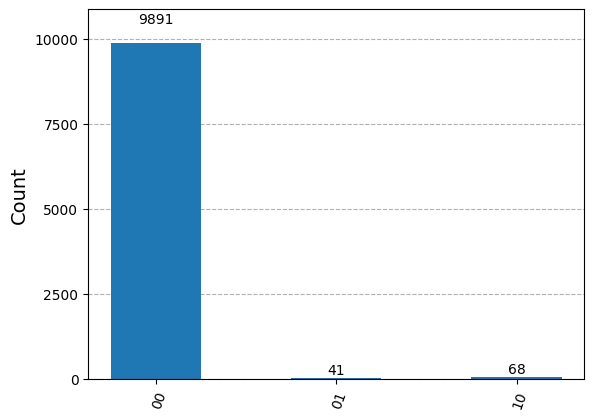
\includegraphics[width=\linewidth]{Images/deutsch_jozsa_const_0results.png}
        \caption{$f = f_1 \Rightarrow$ constant}
        \label{fig:deutsch_jozsa_result_f1}
    \end{subfigure}
    \hfill
    \begin{subfigure}[b]{0.45\linewidth}
        \centering
        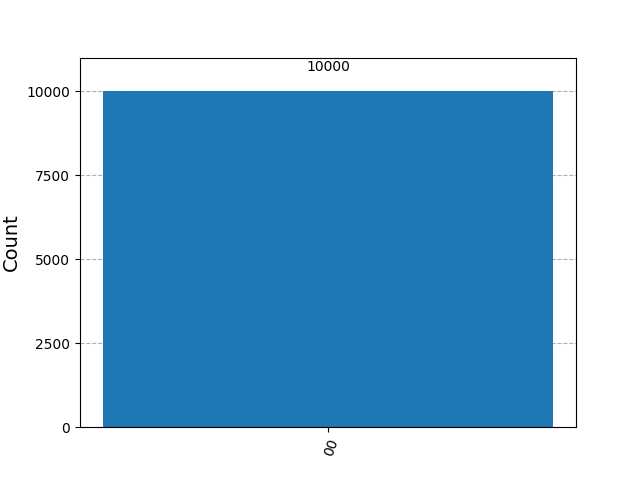
\includegraphics[width=\linewidth]{Images/deutsch_jozsa_const_1results.png}
        \caption{$f = f_2 \Rightarrow$ constant}
        \label{fig:deutsch_jozsa_result_f2}
    \end{subfigure}

    \vspace{0.5cm}

    \begin{subfigure}[b]{0.45\linewidth}
        \centering
        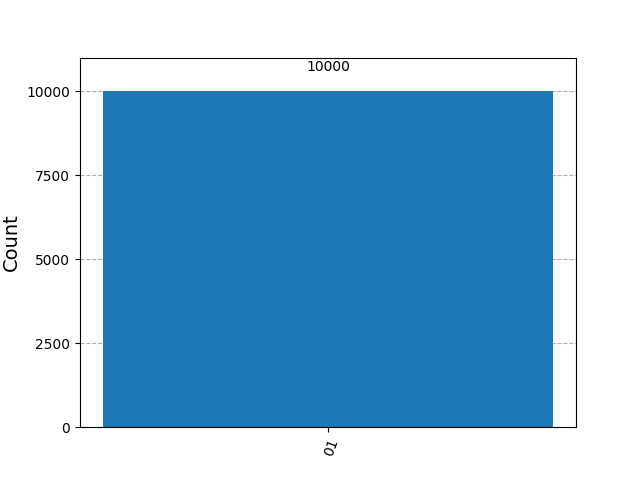
\includegraphics[width=\linewidth]{Images/deutsch_jozsa_bal_0result.png}
        \caption{$f = f_3 \Rightarrow$ balanced}
        \label{fig:deutsch_jozsa_result_f3}
    \end{subfigure}
    \hfill
    \begin{subfigure}[b]{0.45\linewidth}
        \centering
        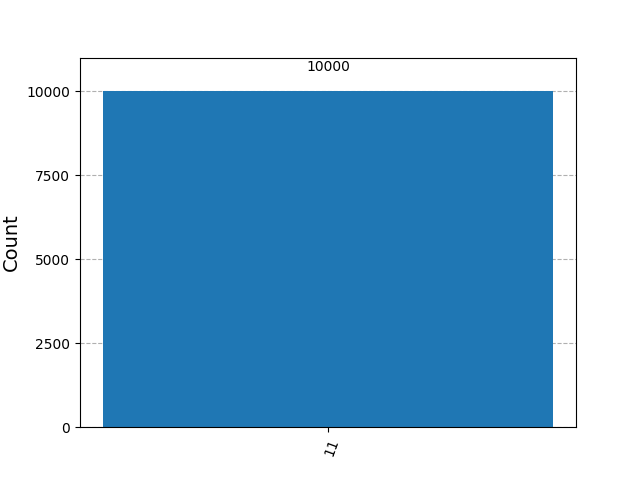
\includegraphics[width=\linewidth]{Images/deutsch_jozsa_bal_1result.png}
        \caption{$f = f_4 \Rightarrow$ balanced}
        \label{fig:deutsch_jozsa_result_f4}
    \end{subfigure}

    \caption{Deutsch-Jozsa algorithm results for various functions.}
    \label{fig:deutsch_jozsa_results}
\end{figure}

As seen in Figure~\ref{fig:deutsch_jozsa_result_f1}, the measurement outcome of the first two qubits is \texttt{00} (observed 9891 times out of 10,000 shots). This confirms that the function implemented inside the oracle was a constant function, as expected. Similar conclusions can be drawn from the other subfigures: each result aligns well with the type of function (constant or balanced) that was implemented.

\end{enumerate}
It is important to note that the Deutsch-Jozsa algorithm allows us to determine whether a function is constant or balanced, but not to identify the specific function out of the possible options. Specifically, we observe that the outcome is $0^n$ only when the function is constant. For balanced functions, the resulting state is always orthogonal to $0^n$, and hence measurement never yields $0^n$.

Due to hardware noise and the probabilistic nature of quantum mechanics, results may vary slightly across different runs. However, the outcome distribution will still reflect the expected pattern, distinguishing constant from balanced functions.

This method can be generalized to circuits with any number of qubits. We can construct corresponding oracles for any constant or balanced function, optimize the circuit, and run it to obtain reliable results.

Finally, note that in practice, the oracle is usually treated as a black box. We do not concern ourselves with its internal structure—only with its effect on the quantum state. As established earlier, any classical function can be implemented within a quantum circuit, so the focus of the algorithm is on using the oracle, not constructing it.


